\documentclass[usletter, 12pt]{article}
 
\usepackage{../VB}
\usepackage{cleveref}
\usepackage{caption}

%\doublespacing

\begin{document}

\lhead{\textsc{Causal Exaggeration}}

\selectlanguage{english}
	
	\title{Causal Exaggeration:\\ Unconfounded but Inflated Causal Estimates}

	\author{Vincent Bagilet
		\thanks{Columbia University, New York, USA. Email: \url{vincent.bagilet@columbia.edu}. 
			A previous version of this paper was co-authored with Léo Zabrocki-Hallak; I cannot thank him enough for his invaluable contributions to the project. I am very grateful to Hélène Ollivier and Jeffrey Shrader for their guidance and thank Sylvain Chabé-Ferret, Jesse McDevitt-Irwin, David McKenzie, José Luis Montiel Olea, Suresh Naidu, Claire Palandri, Stephan Thies and Roberto Zuniga Valladares for helpful comments, as well as lab members at Columbia and seminars participants at Columbia, IPWSD, the Paris School of Economics and the Toulouse School of Economics.}
	}
	
	\institution{Sustainable Development PhD Program, Columbia University}

	\date{February 21, 2023}
	
	
	\maketitle
	
	\begin{center}
		\large \textsc{\textbf{Abstract}}\\
	\end{center}
		
		The credibility revolution in economics has made causal inference methods ubiquitous. At the same time, an increasing amount of evidence has highlighted that the literature strongly favors statistically significant results. I show that these two phenomena interact in a way that can substantially worsen the reliability of published estimates: even when causal identification strategies successfully reduce bias caused by confounders, they can decrease statistical power and create another type of bias, leading to exaggerated effect sizes. This exaggeration is consequential in environmental economics, as cost-benefit analyses turn estimates into decision-making parameters for policy makers. I characterize this trade-off using a formal mathematical derivation and realistic Monte Carlo simulations replicating prevailing identification strategies. I then discuss potential avenues to address it. 
		
		%To avoid confounding, causal identification strategies focus on a subset of the variation in the data; the plausibly exogenous part. In this paper, I argue that this can reduce statistical power and lead estimates to exaggerate true effects sizes. Using realistic Monte Carlo simulations and a mathematical derivation, I show that for the main causal strategies, a perfectly convincing identification does not guaranty an absence of ``bias'' and that improving identification can actually pull us away from the true effect. I then discuss potential avenues to address this issue.
		
		%Quasi-experimental studies make empirical economics credible. To avoid confounding, causal identification strategies focus on a subset of the variation in the data, the plausibly exogenous part. In this paper, I argue that it can reduce statistical power and lead published estimates to exaggerate true effects sizes. Using realistic fake data simulations and a mathematical derivation, I show that %for the main causal strategies, there can be a trade-off between confounding and exaggeration: we may avoid a bias at the risk of generating another one.
		%using the main causal identification strategies to avoid a bias can also generate another one. I then discuss potential avenues to address this issue.\\~\\
	
	\begin{center}
		\Large \textsc{\textbf{Preliminary introduction}}\\
	\end{center}
	
	
	\newpage
	
	\section{Introduction}
			 	 		
		
					One of the main challenges of empirical economics is identifying causal effects. Identifications strategies such as Regression Discontinuity (RD), Instrumental Variables (IV), Difference-in-Differences (DiD) and event studies help us achieve this goal. To do so, these strategies only use a portion of the variation in the data. They exploit the exogenous part of the variation in the treatment or decrease the sample size by only considering observations for which the as-if random assignment assumption is credible. This reduction in the variation used can decrease precision and thus statistical power---the probability of rejecting the null hypothesis when it is false, or put simply, the probability of obtaining a statistically significant estimate. There is, therefore, a tension between reducing confounding and statistical power.
			
			When statistical power is low, not only is the estimator imprecise but statistically significant estimates exaggerate the true effect size \citep{gelmanType2000, ioannidis_why_2008, gelman_beyond_2014}. Only estimates at least 1.96 standard errors away from zero are statistically significant at the 5\% level. In under-powered studies, these estimates make up a selected sub-sample of all estimates, located in the tails of the distribution of all possible estimates. The average of these statistically significant estimates differs from the true effect, located at the center of the distribution if the estimator is unbiased. They exaggerate the true effect and the less precise the estimator, the larger exaggeration is.  \Cref{fig:graph_exag} illustrates the inflation of significant estimates caused by imprecision. When power is low, obtaining a statistically significant estimate from an unbiased estimator does not guarantee that it will be close to the true effect. An estimator $\hat{\beta}$ of the true effect $\beta$ might be unbiased in the traditional sense of $\mathbb{E}[\hat{\beta}] = \beta$ but conditionally biased in the sense that $\mathbb{E}[\hat{\beta} | \text{ Significant}] \neq \beta$. For statistically significant estimates, the tension between statistical power and reducing confounding is thus a tension between reducing confounding and exaggerating the true effect size.
			
			   \begin{figure}[!h]
				\begin{center}
					\caption{Significance and distribution of two unbiased estimators with different variances}
					\label{fig:graph_exag}
					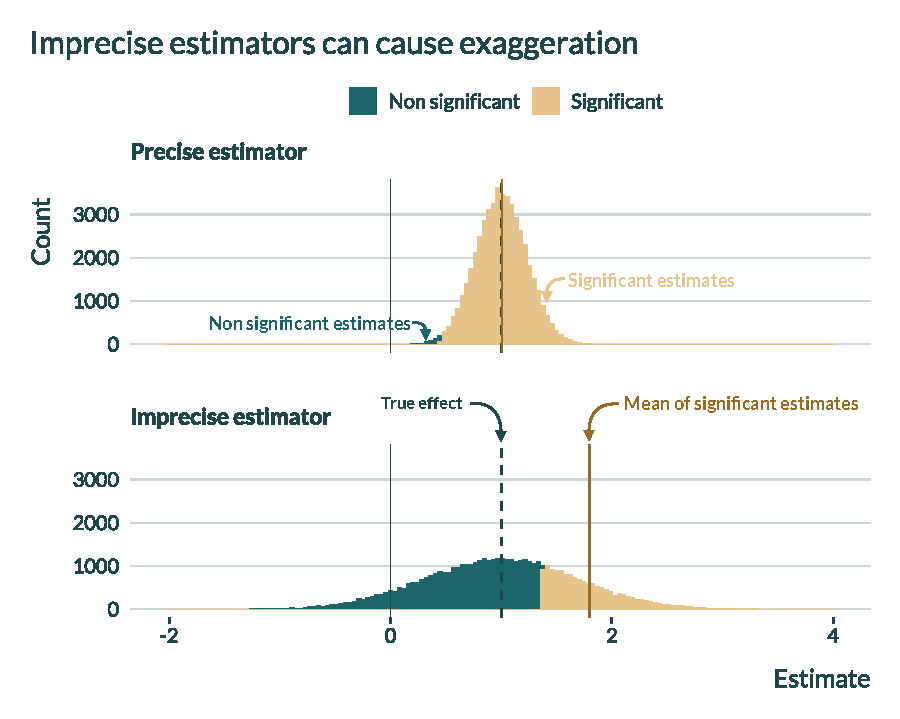
\includegraphics[width=0.8\linewidth]{images/graph_intuition_precision.pdf}
					\caption*{\footnotesize \textit{Notes}: 100,000 draws from two normal distributions $\mathcal{N}(1, 0.05)$ and $\mathcal{N}(1, 0.5)$. Significance level: 5\%}
				\end{center}
				\vspace{-1cm}
			 \end{figure}
			
			Yet, exaggeration only arises under two conditions: 1) a publication bias favors statistically significant results and 2) statistical power is low. A large body of literature underlines that the economics literature selects results based on statistical significance \citep[for instance]{rosenthal_file_1979, brodeur_star_2016, andrews_identification_2019, abadie_statistical_2020, brodeur_methods_2020}. Additional studies have highlighted its frequent and substantial lack of statistical power and resulting exaggeration \citep{ioannidis_power_2017, ferraro_featureis_2020}. %Under-powered studies can therefore produces estimates that exaggerate true effect sizes. 
			Even in experimental economics, with a high level of control and an arguable absence of confounders, studies from top economics journals failed to replicate, the original estimates being on average inflated by a factor of at least 1.5 \citep{camerer_evaluating_2016}. In the non-experimental economics literature, where statistical power is rarely a central consideration under current practices, several meta-analyses provide evidence of consequential exaggeration. \cite{ioannidis_power_2017} finds that the median statistical power in a wide range of areas of economics is no more than 18\%. Despite %the widespread use of convincing causal identification strategies and 
			usually large sample sizes, they show that nearly 80\% of estimates are likely exaggerated by a factor of two. 
			 %In environmental economics, using a more conservative approach, \cite{ferraro_featureis_2020} finds that 56\% of estimates are exaggerated by a factor of two or more. I provide evidence of exaggeration in a subfield of this literature, that on the acute health effects of air pollution in a companion paper \citep{bagilet_accurate_2023} and further expand this analysis in the present paper.  
			As further illustrated in section \ref{lit_review}, the magnitude of exaggeration can be considerable and in some situations could be on par with that of a bias caused by confounders.
			%especially in settings where bias caused by confounders may not be as large. For example, Weidmann and Miratrix (2021) documents and absence of evidence of selection bias due to unobservables in the evaluations of school programs they investigate.
			%Add CBA thing here
			Taking exaggeration into account and to understanding its drivers is therefore crucial.
			%In environmental economics, where estimates are often directly used to inform policies, in particular via CBA, obtaining accurate estimates is even more crucial. In this field, we often chase small and diffuse effects, that are intrinsically difficult to capture, often because playing a role in the long term or being causaly diffuse. 
			%It is even more important in some fields such as environmental economics where estimates are used to directly inform public policy. Via CBA 
			
			 Accurate point estimates are instrumental as they often inform policy decisions through Cost-Benefit Analyses (CBA). For instance, environmental economics estimates enter the computation of the Social Cost of Carbon or routinely help policy makers decide of the implementation of regulations. Yet, the underlying effects can be relatively small and thus difficult to capture, making the studies subject to exaggeration. Estimates of the impact of environmental regulations on job losses constitute a good example \citep{gray_environmental_2023}. For instance, \cite{walker_environmental_2011} documents the impact of the Clean Air Act amendments of 1990 on employment and finds an effect of -14.2\% (s.e. 4.3). For similar policies, other studies find smaller effects, of the order of magnitude of -3\% \citep{greenstone_impacts_2002, gray_environmental_2023}. The design of \cite{walker_environmental_2011} would not be precise enough to retrieve an effect size of this magnitude. If the true effect was in fact of this magnitude, the statistical power of the study would be 11\% and significant estimates would exaggerate the true effect by a factor of 3.5 on average. In this example, bias caused by exaggeration would be substantial and could have detrimental policy implications.\footnote{Of course, in the particular setting of \cite{walker_environmental_2011}, the true effect might be larger than 3\%. I am not claiming that the study is flawed but instead that its level of precision would produce inflated significant estimates if the true effect was of the order of magnitude of 3\%.}
			
			% goal of this study
			In the present paper, I argue that the use of causal identification strategies increases exaggeration. %I propose an overarching mechanism that may contribute to do so. 
			Reviewing a literature, using a mathematical derivation and Monte Carlo simulations, I show that design choices in quasi-experimental studies can be seen as a trade-off between avoiding confounding and overestimating true effect sizes. To limit the threat of confounding, causal inference methods discard variation and therefore reduce statistical power. When combined with a statistical significance filter, this results in exaggeration bias. While causal identification strategies are essential to describe causal relationships, the present paper emphasizes that a perfectly convincing identification does not guaranty an absence of ``bias'' and that improving identification can actually pull us away from the true effect. The same strategies which remove bias caused by confounding actually introduce another type of bias. 
			
			%mechanisms
			%I analyze the key factors affecting the confounding-exaggeration trade-off for a wide range of identification strategies : RD, IV, event studies, strategies such as DiD relying on  fixed effects (FEs) or generic controls and matching. 
			
			%IMPORTAAAAAANNNNTTT
			%Maybe change order
			All causal identification strategies discard variation in order to identify causal effects but the confounding-exaggeration trade-off is mediated through a distinctive channel for each of them. RD designs discard part of the variation by only considering observations within the bandwidth, decreasing the effective sample size and thus precision. An IV strategy only uses the subset of the variation in the treatment that is explained by the instrument. In studies leveraging exogenous shocks, the variation used to identify an effect sometimes only comes from a limited number of treated observations. Approaches that do not actually leverage natural experiments but aim to identify a causal effect by controlling for confounders also limit the variation used. 
			%When all confounders are arguably measured, matching has a causal interpretation but it still 
			Matching prunes units that cannot be matched and thus reduces the effective sample size. 
			Adding controls or fixed effects can increase the variance of the estimator and exaggeration if they absorb more of the variation in the treatment than in the outcome variable. 
			
			%IMPORTAAAAAANNNNTTT
			%I need to change and strengthen that: reorganize with the right id strats
			Since causal identification strategies can be interpreted as ways of controlling for confounders, this last point actually ties all the strategy-specific arguments together.\footnote{Fixed Effects (FEs) based identification strategies such as DiD control for the invariant, unobserved, and arguably endogenous part of the variation in the outcome. An IV approach essentially partials out the variation in $x$ unexplained by the instruments. %as made more explicit in the Control Function (CF) approach to the IV. the predicted residuals of the regression of the endogenous variable of interest on the instrument.
			 Fuzzy-RD and propensity score matching can be thought of as control function approaches, of the forcing variable and propensity score respectively. In addition, excluding observations that are outside the bandwidth or unmatched is equivalent to controlling for observation-level fixed effects for these observations.} When these identification strategies absorb more of the variation in the treatment than in the outcome, they increase the variance of the resulting estimator and can cause exaggeration. 
			 %maths_intro_starts
			 Considering a simple linear homoskedastic model gives the intuition for this trade-off between exaggeration and omitted variable bias (OVB) for control approaches.  Let $y_{i} = \alpha + \beta x_{i} + \delta w_{i} + u_{i}$, $\forall i \in \{1, .., n\}$,  with $x$ the variable of interest, $w$ a potentially unobserved variable correlated with $x$ and $u$ an error term. Under usual assumptions and using the Frisch-Waugh-Lovell theorem, we get that $ \sigma_{\hat{\beta}_{\textsc{ovb}}}^2$ and $ \sigma_{\hat{\beta}_{\textsc{ctrl}}}^2$, the variance of the estimators for $\beta$ when omitting $w$ (short regression) and controlling for it (long regression) are respectively:
			~
			\[
				\sigma_{\hat{\beta}_{\textsc{ovb}}}^2 =
				 \dfrac{\sigma^{2}_{u_{\textsc{ovb}}}}{n \ \sigma_{x}^{2}} =
				 \dfrac{\sigma^{2}_{y^{\perp x}}}{n \ \sigma_{x}^{2}}
				 \qquad \text{and} \qquad
				 \sigma_{\hat{\beta}_{\textsc{ctrl}}}^2 = 
				 \dfrac{\sigma^{2}_{u_{\textsc{ctrl}}}}{n \ \sigma_{x^{\perp w}}^{2}} =
				  \dfrac{\sigma^{2}_{y^{\perp x, w}}}{n \ \sigma_{x^{\perp w}}^{2}}
			\]
			
			where $\sigma^{2}_{u_{\textsc{ovb}}}$ and $\sigma^{2}_{u_{\textsc{ctrl}}}$ are the variances of the residuals in the regression of $y$ on $x$ and of $y$ on $x$ and $w$ respectively or equivalently the variances of the parts of $y$ that are orthogonal to $x$ and to $x$ and $w$ respectively ($\sigma^{2}_{y^{\perp x}}$ and $\sigma^{2}_{y^{\perp x, w}}$), $\sigma^{2}_{x}$ is the variance of $x$ and $\sigma^{2}_{x^{\perp w}}$ is the variance of the part of $x$ orthogonal to $w$. Thus,
			
			\[
				\sigma_{\hat{\beta}_{ovb}}^2 <  \sigma_{\hat{\beta}_{ctrl}}^2
                   		\quad \Leftrightarrow \quad 
				\dfrac{\sigma^{2}_{y^{\perp x}}}{n \ \sigma_{x}^{2}} < \dfrac{\sigma^{2}_{y^{\perp x, w}}}{n \ \sigma_{x^{\perp w}}^{2}}
				\quad \Leftrightarrow \quad 
				\dfrac{\sigma^{2}_{x^{\perp w}}}{\sigma_{x}^{2}} <
				\dfrac{\sigma^{2}_{y^{\perp x, w}}}{ \sigma_{y^{\perp x}}^{2}}
			\]
			
			Controlling for $w$ will increase the variance of the estimator if the fraction of the variance unexplained by $w$ is greater for $y^{\perp x}$ than for $x$. Put differently, if controlling absorbs more of the variation in $x$ than in the residual part of $y$ ($y^{\perp x}$), it will increase the variance of the estimator.  Since exaggeration increases with the variance of the estimator, controlling for a confounder can increase exaggeration.
			This has direct implications when using fixed effects: an exaggeration bias can arise from the use of fixed effects if they absorb more of the variation in $x$ than in $y^{\perp x}$. %FIND EXAMPLES !! ---which can often be the case in settings such as regression of agricultural yield on weather variables or ---
			 Under some circumstances discussed in sections \ref{maths} and \ref{simulations}, controlling can even produce an exaggeration bias larger than the OVB that would result from an absence of controls. 
			
			% what we actually do
			In the remainder of the paper, I first document the magnitude of the trade-off. To do so, I build on existing literature reviews to discuss evidence of exaggeration bias in a large set of causal studies mostly published in top journals \citep{brodeur_methods_2020, youngConsistencyInferenceInstrumental2022, bagilet_accurate_2023, lalHow2024}. %I then focus on IV designs as they allow for a within-study comparison between causal and non-causal estimates, the Two-Stage Least-Squares (2SLS) and the corresponding  ``naive'' Ordinary Least Squares (OLS) respectively. %IVs often reduces precision, limits statistical power to the point that 2SLS estimates reject the OLS point estimate and are not able to provide strong evidence supporting that the OLS is biased \citep{youngConsistencyInferenceInstrumental2022}. 
			These analyses reveal heterogeneity across analyses: while exaggeration might be limited in some studies, it is likely substantial in many others. 
			%They would not be able to accurately retrieve effect size of the magnitude of the OLS estimate and significant results would overestimate it.
			%By reducing precision, IVs---and causal identification strategies in general---likely induce exaggeration and produce biased significant estimates: 
			In the set of IV papers reviewed in \cite{youngConsistencyInferenceInstrumental2022}, I show that 
			%less than 10\% of the designs would retrieve an effect size equal to that of the ``naive'' OLS---at the conventional 80\% power threshold. This proportion increases to 17\% for headline results. 
			half of the designs would exaggerate a true effect size of the magnitude of the ``naive'' OLS estimate by a factor larger than 3.2---and by a factor larger than 2.0 for headline designs. %Similarly, in the literature on the short term health effects of air pollution that I review in \cite{bagilet_accurate_2023}, only 2\% of the IV designs would retrieve an effect size equal to that of the ``naive'' OLS and the median exaggeration factor would be 4.5. 
			For an example study, I directly compare confounding and exaggeration biases and show that in this study the bias of the IV could be larger than that of the OLS and that exaggeration may explain this difference. 
			
			Next, I derive a formal proof of the existence of the trade-off for prevailing causal identification strategies. Specifically, I show that the bias caused by exaggeration can be larger than the one caused by confounders. I also analyze the drivers of exaggeration and demonstrate that it increases as the strength of the instruments decreases, the number of exogenous shocks decreases or when controlling for a confounder absorbs more of the variation in the treatment than in the outcome. 
			
			 Then, I show that this ``causal exaggeration'' arises for realistic parameter values by further exploring its drivers in realistic settings.
			 % using examples drawn from environmental, education, labor, health and political economics. 
			 %We show that an actual trade-off between exaggeration and confounders can exist as exaggeration can be large for research designs implemented in actual studies. 
			The exaggeration of statistically significant estimates can be defined as the absolute value of the ratio of these significant estimates over the true effect, a quantity which is never known in a real world setting. In order to be able to compute this quantity, I turn to simulations. Monte-Carlo simulations also allow varying the value of the parameter of interest \textit{ceteris paribus}, something that would not be possible otherwise. To make these simulations concrete, I calibrate them to emulate existing studies from environmental, education, labor, health and political economics. %All other simulation assumptions are chosen to facilitate the recovery of the effect of interest: I consider simple linear models with constant and homogenous treatment effects, \textit{i.i.d.} observations and homoskedastic errors. All the models are correctly specified and accurately represent the data generating process, except for the omitted variable. 
			I find that causal exaggeration can be substantial in realistic settings where the variation remaining for identification is limited. 
									
			Finally, I discuss concrete avenues to address causal exaggeration when carrying out a non-experimental study\footnote{In experimental studies, there are essentially no confoundings. A solution to increase power and reduce exaggeration is generally to increase sample size, reduce noise by improving measurement or improving balance or to focus on larger potential effects.}. A series of tools can be used to evaluate the potential magnitude of confounding and exaggeration issues separately. Sensitivity analyses help with the former while power calculations help with the latter. %These power calculations can be computed before and after the analysis is carried out. 
			%For instance, the sensitivity analysis tools developed in \cite{cinelli_making_2020} enable to assess how strong confounders would have to be to change the estimate of the treatment effect beyond a given level we are interested in. 
			Considering the attention given to bias avoidance in the economics literature, I underline that making power central to non-experimental analyses, even after an effect has been found, would help limiting bias caused by exaggeration. Prospective power simulations help identify the design parameters affecting power and exaggeration by approximating the data generating process \citep{gelman_regression_2020, black_simulated_2022}. Retrospective power calculations allow evaluating whether a study would have had enough power to confidently estimate a range of smaller but credible effect sizes \citep{gelman_beyond_2014, stommes_reliability_2021}.
			%%%%%%%% Evaluating potential exaggeration and confounders is however complex as both rely on unobserved shit
			Focusing more specifically on the trade-off and its drivers, I consider tools to identify the variation actually used for identification when using causal identification strategies. %The \href{https://vincentbagilet.github.io/causal_exaggeration/}{companion website} describes in details how such analyses can be implemented. Finally, I briefly discuss potential solutions to mitigate this trade-off.
						
			% first contribution
			This paper contributes to three strands of the applied economics literature. First, the idea that causal identification estimators, while unbiased, may be imprecise is not new; this is part of the well-known bias-variance trade-off \citep{imbens_optimal_2012, deaton_understanding_2018, hernan_causal_2020, ravallion_should_2020}. I approach this literature from a different angle: through the prism of statistical power and publication bias. Not only the limited precision resulting from the use of causal identification methods could make it difficult to draw clear conclusions regarding the exact magnitude of the effect but I argue that it might also inherently lead to inflated published effect sizes, creating another ``bias''. The bias-variance trade-off can in fact be a bias-bias trade-off.
			
			% second contribution
			Second, studies discussing the exaggeration of statistically significant estimates due to a lack of power usually do not investigate its determinants or focus on specific causal identification methods separately \citep{ioannidis_power_2017, schellEvaluatingMethodsEstimate2018, ferraro_featureis_2020, black_simulated_2022, stommes_reliability_2021, arel-bundockQuantitativePoliticalScience2022}.  In a companion paper, I highlight tangible design parameters that can cause exaggeration for a wide range of empirical designs \citep{bagilet_accurate_2023}. In the present paper, I take a step back and propose an overarching mechanism, inherent to causal identification strategies as a whole, and that can explain these issues: although each strategy does so through different means, in essence they discard part of the variation, thereby increasing the risks of exaggeration. %This connection could be exacerbated by the fact that, as noted by \cite{brodeur_methods_2020}, publication bias is more prevalent for some methods such as the IV. 
			
			% third contribution
			Third, this study contributes to the literature on replicability in economics \citep{camerer_evaluating_2016, ioannidis_power_2017, christensen_transparency_2018, kasy_forking_2021}. The trade-off presented in this paper suggests that the widespread use of convincing causal identification methods in economics may not shield the field from potential replication threats.
			%The trade-off presented in this paper may contribute to explaining the replication failures observed in empirical economics, despite the widespread use of convincing causal identification methods.
			
			In the following section, I document evidence of causal exaggeration in the causal  economics literature. In section \ref{maths}, I study the drivers of exaggeration and formally show in a simple setting that the use of causal identification strategies can exacerbate it. In section  \ref{simulations}, I implement realistic Monte-Carlo simulations to illustrate the existence of the confounding-exaggeration trade-off. I discuss potential solutions to navigate this trade-off in section \ref{discussion} and conclude in section \ref{conclusion}.
	
	
		
			
	\newpage
	
\bibliographystyle{agsm}
\bibliography{causal_inflation}	
	
	
	
	
	
	
		
\end{document}